% Template for Biophysics paper in LaTeX
%
% To compile into a document, run
% latex biophys_latex_template
% bibtex biophys_latex_template (if bib file and bst file is included in TeX file)
% latex biophys_latex_template (run 2-3 times repeatedly)
% dvips biophys_latex_template.dvi
%
% or replace the latex command by the pdflatex command in the lines above to
% generate a PDF file and use acroread or xpdf for viewing and
% printing instead of the postscript generating program dvips

% Use standard biophys document class with default font size
% and typeset in one column. If you need to typeset in two column
% then give the option "twocolumn" ie \documentclass[twocolumn]{biophys}
\documentclass[twocolumn]{biophys}
\usepackage{helvet,times}
\usepackage{bm,textcomp}

\jno{kxl015} %journal number
\gridframe{N}%option for grid around the text "Y" or "N"
\cropmark{N}%option for cropmark around the text "Y" or "N"

\doi{doi:15}% DOI number in the copyright line

%The first page number and last page number automatically generated.
%To change the page number \setcounter{page}{10} automatically reset
%the first and last page number but two times compilation required.
%If you want to edit the page range in catch line
% then edit the below two lines
%\fpage{}
%\lpage{}
%For update volume number, activate below command
%\volume{00}
%For update issue number, activate below command
%\issue{00}
%For update Month, activate below command
%\Month{Month}
%For update Year, activate below command
%\Year{Year}


% Packages to load (all standard on a modern LaTeX system on Linux)

% Make doublespaced ugly typography required for mysterious
% reasons by most journals - comment out for normal output
%\usepackage{setspace}
%\doublespacing
% AMS-Math package to have nice multi-line equations and other goodies
\usepackage{amsmath}
% Show labels for easy orientation, comment out for final version
% \usepackage{showlabels}

% EPS/PDF graphics
% Place figures in the document directory in both the EPS and PDF
% formats, e.g., fig_1.eps and fig_1.pdf. Use the includegraphics
% command without file extension, e.g. \includegraphics*[width=3.25in]{fig_1}
% The pdflatex or latex programs then work automagically with the
% appropriate formats.  EPS figures can be converted to PDF using
% the epstopdf program present on most Linux disributions. Epstopdf and graphicx
% are included in biophys class file.
% \usepackage{graphicx}

% Citation style in the text: numbers in parenthesis, sorted by their
% order in the list of references.
% Uses a range if possible: (1-3), not (1,2,3)

\usepackage{algorithm}
\usepackage[noend]{algpseudocode}
\usepackage{caption}
\usepackage{subcaption}
\usepackage{graphicx}

\usepackage[round,numbers,sort&compress]{natbib}

% Bibliography style (requires the style file biophysj.bst in the
% document directory)

%\bibliographystyle{biophysj}

% Numbering style in the list of references: a number followed by a period

\renewcommand{\bibnumfmt}[1]{#1.}

% Examples of special definitions (amsmath package required)
\newcommand{\erf}{\operatorname{erf}}        % error function
\newcommand{\erfc}{\operatorname{erfc}}      % complementary error function
\newcommand{\BibTeX}{\textsc{Bib}\TeX}       % corect BibTeX appearance
\makeatletter
\def\BState{\State\hskip-\ALG@thistlm}
\makeatother


% Running head


\markboth{Biophysical Journal: Biophysical Letters}{Biophysical Journal: Biophysical Letters} %for running head

% We are done with the headers, the actual document starts here




\begin{document}



\setcounter{page}{1} %first page number

\title{Modelling of mRNA transport in \textit{Drosophila} nurse cells}


\author{Jonathan Harrison, Richard Parton, Ruth Baker}

\address{University of Oxford}


% generate the title page from the info in the headers above


%Abstract environment needs 3 arguments. They are
%1. The abstract
%2. Received date
%3. Address, email

\begin{abstract}%
{Insert abstract information here}%1
{Insert Received for publication Date and in final form Date.}%2
{Insert Corresponding address and emails}%3
\end{abstract}

\maketitle %%The above information typeset through this command

\section{Introduction}

The localization of mRNA is crucial in a variety of biological contexts for the targeting of proteins to their site of function.
%This enables proteins to be
This method of gene expression is particularly relevant for polarized cells such as oocytes and early embryos.
For example, the axes of \textit{Drosophila Melongaster} are established through regulation of gradients in \textit{bicoid} (\textit{bcd}), \textit{gurken} (\textit{grk}), \textit{oskar} (\textit{osk}) and \textit{nanos} (\textit{nos}) mRNA \citep{wolpert1998}.
mRNA localization has been observed in a variety of species and cell types, including Drosophila and Xenopus oocytes, neurons, chicken fibroblasts, yeast and bacteria \citep{wilkie2001drosophila, bobola1996asymmetric, mowry1992vegetal, rosbash1993rna, nevo2011translation}, thus demonstrating that this process is ubiquitous and not limited to large cells. 
Drosophila rely heavily on asymmetric locatization of mRNAs to coordinate the early development process both spatially and temporally.

Recent advances in imaging techniques and image analysis technologies \citep{jeffery1983localization, bertrand1998localization, hamilton2010particlestats} have allowed an advancement of our understanding of the mechanisms of mRNA localization. 
The use of flourescence in situ hybridisation (FISH) enables single molecules of mRNA to be labelled with high levels of sensitivity and specificity. 
The development of the MS2-MCP system, which consists of a MS2 bacteriophage RNA stem loop bound by MS2 coat protein fusion to a flourescent protein \citep{parton2014subcellular}, has had great benefits for the imaging of live cells \textit{in vivo}.
The MS2-MCP system has been used successfully in the visualisation of \textit{nos}, \textit{grk}, \textit{bcd} and \textit{osk} mRNAs in Drosophila \citep{forrest2003live, jaramillo2008dynamics, weil2006localization, zimyanin2008vivo}.
Although there are limitations to these technologies dependent on cell type, they have permitted an improvement of our understanding of intracellular motility and structure.
What has become clear is that a variety of different mechanisms are used to ensure localization of mRNAs.

\subsection{Outline of mRNA localization process}

Once mRNA has been transcribed from DNA in the nucleus, the process by which it reaches its final site of localization, where it is then translated into protein, can be divided into four main stages: particle formation; nuclear export; transport; and anchoring.
We will address each of these processes in turn.

mRNA does not exist on its own inside the cell.
Instead the mRNA binds to proteins to form particle complexes, which are also known as ribonuclearproteins (RNPs). 
These proteins perform a range of different functions, including translational regulation to prevent translation while the mRNA is in transit, and may determine the final destination of the particle \citep{hamilton2013multidisciplinary}.
Examples of proteins that form these paricles include \textit{Squid} (\textit{sqd}) and \textit{Orb}.
There is also evidence that RNPs are dynamically remodelled during the transport process \citep{weil2012drosophila}.

After the RNA has formed into RNPs, it must diffuse through the crowded interchromatin spaces in the nucleus until it reaches a nuclear pore complex (NPC).
The RNP is then exported out of the NPC into the cytoplasm via interactions with co-factors.
Certain NPCs are more active than others at different times \citep{weil2012drosophila}, but the overall direction of export out of the nucleus is unbiased \citep{wilkie2001drosophila}. 

The transport stage of mRNA localization occurs by different mechanisms for different mRNAs.
The most common method observed is transport via molecular motors moving along the cytoskeleton (either microtubules or actin filaments). 
However, \textit{nos} mRNA localizes using a diffusion and trapping technique \citep{forrest2003live} rather than by active transport. 
Active transport results in faster directed motion with velocities of the order of $1 \mu \text{m} \text{s}^{-1}$ \citep{weil2006localization, zimyanin2008vivo}, which is an order of magnitude quicker than movement by free diffusion.
The motion of RNP complexes on microtubules is often non-uniform in nature, with bidirectionality observed by \citet{vendra2007dynactin} in Drosophila blastoderm embryos.
It should be noted that, conventionally, individual types of molecular motors are thought to move unidirectionally, with Dynein directed towards the minus end of microtubules and Kinesin directed towards the plus end \citep{howard2001mechanics}.
The number of motors required for a given RNP complex can vary and may be governed by cis-acting localization elements in the mRNA \citep{amrute2012single}.
Possible explanations for the bidirectionality include: the bidirectional disorganized distribution of the microtubule network; a tug of war between different molecular motors moving in opposing directions on different microtubules; a tug of war between different motor species all bound to the same RNP complex; reversal of a molecular motor moving on a single microtubule, possibly due to regulation by microtubule associated proteins (MAPs) \citep{buxbaum2015right}. 
The molecular motors must be correctly joined to their cargo and the motor cargo complex secured to the cytoskeleton.
This is ensured by the linkers \textit{Bicaudal D} (\textit{BicD}) and \textit{Egalitarian} (\textit{Egl}) \citep{parton2014subcellular}. 
Although the cytoskeleton was initially thought to be a stable static network, due how it was analysed in fixed material, it has recently been revealed to be a dynamic network with a biased random orientation of microtubules \citep{parton20111}.
This underlying structure had been suggested by the work of \citet{zimyanin2008vivo} who observed RNPs containing \textit{osk} mRNA moving in a biased random walk.  

Once the RNP complex has reached its destination, it must be maintained in position by some anchoring mechanism to keep the mRNA localized within the cell.
\textit{grk} mRNA is anchored by the molecular motor Dynein \citep{delanoue2005dynein} in the Drosophila oocyte and \textit{nos} is trapped by actin \citep{forrest2003live}.
Dynein was observed by \citet{delanoue2005dynein} to act as a static motor without requiring further energy in the form of ATP to function. 
An alternative hypothesis is that continuous active transport is required to ensure the localization of mRNA, since \citet{weil2006localization} found that Dynein motor activity is required to ensure \textit{bcd} localization in the anterior cortex of the Drosophila embryo.

\subsection{Motivation}
After transcription and transport out of the nucleus, many mRNAs are localized and translated in the distinct cytoplasmic domains where they function \citep{jansen2001mrna, parton2014subcellular}.
This process is highly regulated and involves active transport by intricate molecular motors.
mRNA localization is crucial for the establishment of polarity of cells and the formation of the basic animal body plan during development \citep{wolpert1998}. 
It may have importance for a wide range of functions involving memory and learning in the nervous system. 
However, we are a long way from a complete understanding of the mechanisms governing the mRNA cargo transport process.

In particular, mRNA transcripts that set up the \textit{Drosophila} body axes originate in the nurse cells and are actively transported on specialized subpopulations of microtubules into the oocyte through the ring canals \citep{clark2007dynein}.
We will focus on this maternal transfer of transcripts into the oocyte.

One of the challenges involved in live imaging of cells to examine this transport process is the need to scan a sample in three spatial dimensions as well as in time.
This places restrictions on the resolution of data that can be obtained temporally and in the $z$ direction \citep{weil2010making}.
Although there are physical restrictions on what can be achieved by improvements in imaging technologies, these could be overcome by modelling of the transport of mRNA cargos, which may permit sparser sampling in time and finer sampling in space.
This could be achieved by improvements in tracking of individual particles or by considering a more bulk flow approach.
In this way, mathematical modelling could enable us to work with sparse data sets.

\section{Materials and Methods}
\subsection{Modelling approach}
In this context, modelling involves breaking down the mRNA localization process into its key components and identifying the biologically important aspects. 
We will put in place appropriate, simple modelling assumptions to describe the most important parts of the system biologically.
These assumptions must agree with existing experimental observations.

Previous modelling approaches in this area have focused on descriptions of the mechanisms of molecular motors at smaller spatial and and temporal scales \citep{bressloff2013stochastic} or with continuous densities \citep{szymanska2014mathematical} rather than representing single RNP particles.
Other studies have generally considered mRNA dynamics in the oocyte \citep{liu2011role}.
Instead we shall describe the transport of mRNA in the nurse cells surrounding the ooctye, which are connected to each other and to the oocyte via ring canals, using an individual-based stochastic description.

We propose two different approaches to parameterise our model. 
The first will involve direct measurement of parameters, such as the average speed of cargo complexes in active transport.
The second method requires application of an approximate Bayesian computation (ABC) framework \citep{johnston2014interpreting, turner2012tutorial, beaumont2002approximate} to parameterise the model via comparison with certain summary statistics of the data.
This will enable comparison between the experimentally measured parameter values and the posterior for these parameters obtained via ABC.

We aim to produce a testable model in the sense that we are able to make predictions from the model of the result of varying certain parameters, such as the speed of the motor carrying the cargo, which could be tested experimentally using genetic mutants that have behaviour that corresponds to a different value of a given parameter. 
This should inform our understanding of how transcripts transport and localize.

\subsection{Velocity jump process}
The movement of RNP cargos is often described as a biased random walk \citep{zimyanin2008vivo}. Rather than modelling this as a simple random walk in position, we let the direction of motion vary. 
This type of model is known as a velocity jump process and has been successfully applied to directed migration of animals and cells \citep{codling2005calculating, taylorking2015birds}.

\begin{figure}[h]
 \centering
 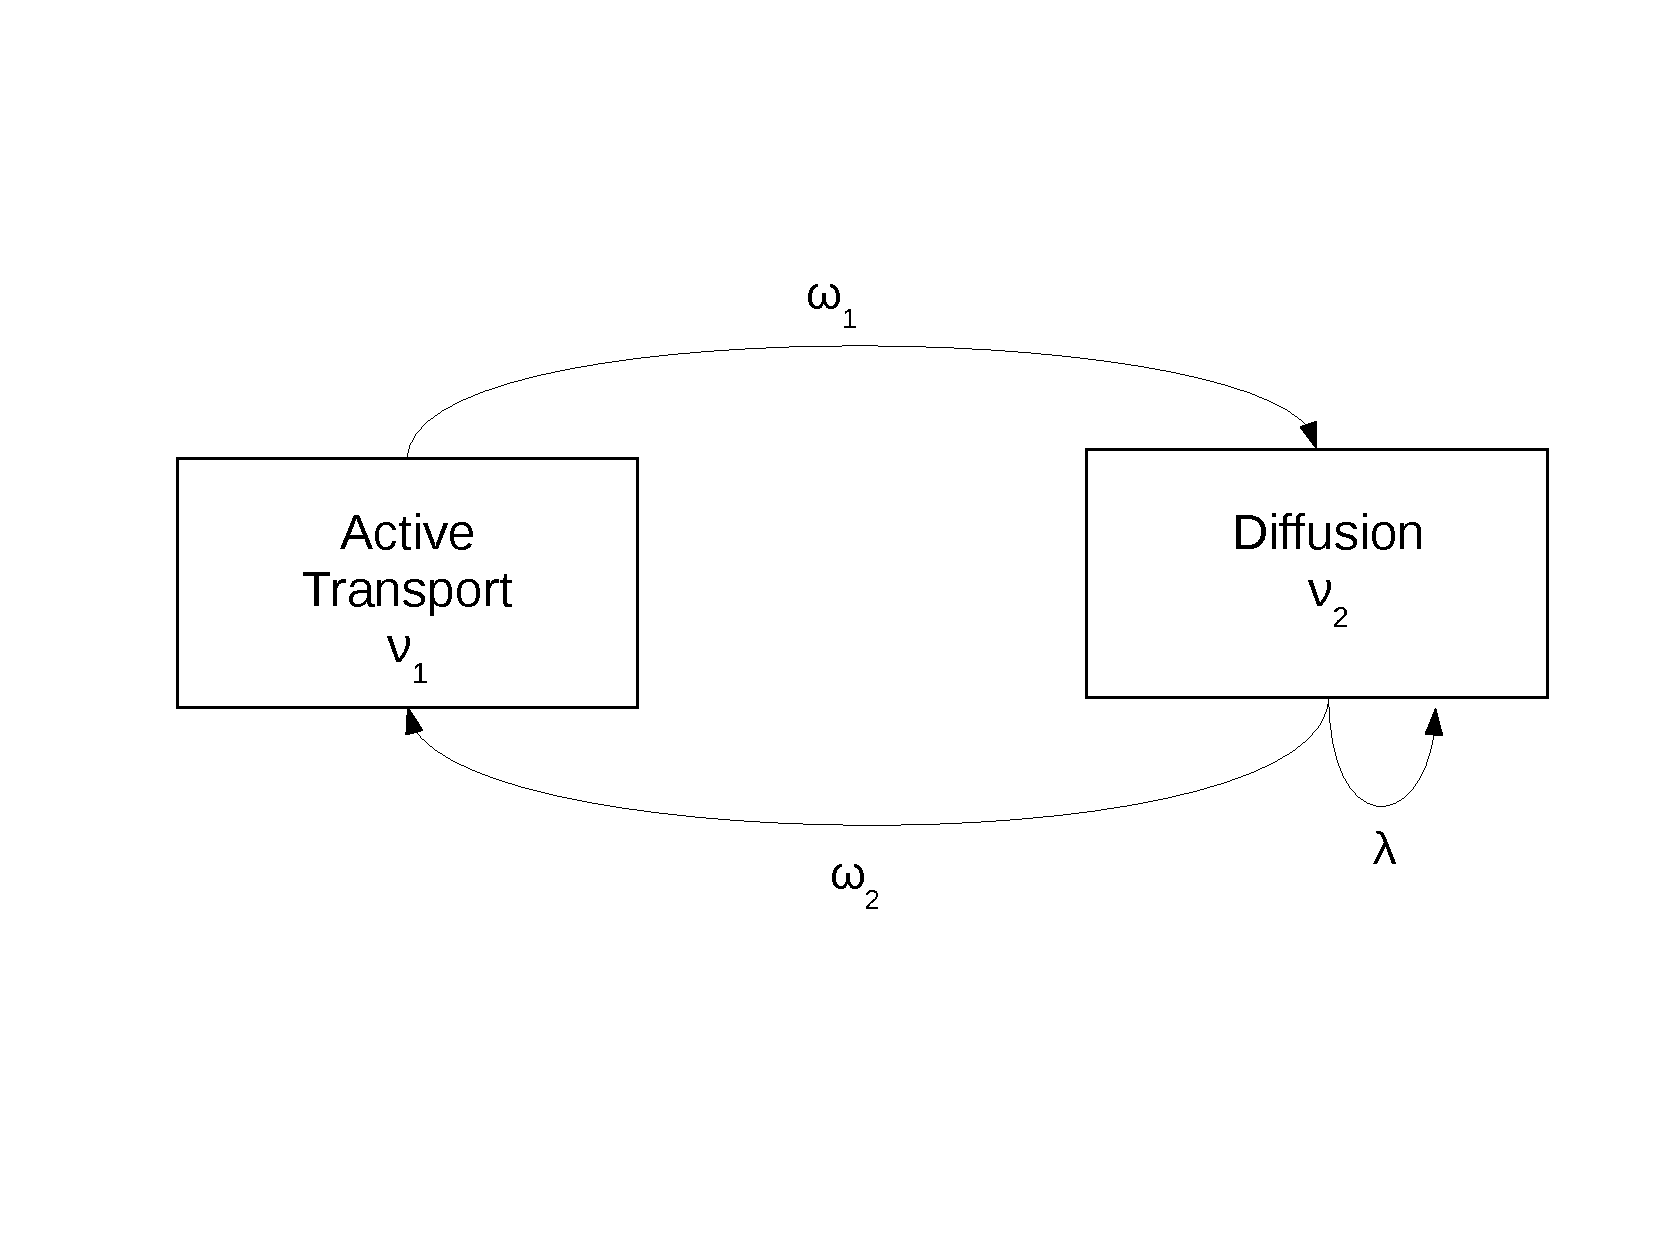
\includegraphics[width=\columnwidth]{/home/harrison/Documents/mRNA/Figures_for_writeup/States_diagram.pdf}
 \caption{States and transitions between the states in the velocity jump process model}
 \label{FIG:Phases_of_motion}
\end{figure}


There are two phases of motion included in the model: an active transport phase when the motor is moving on the microtubules with constant speed $\nu_1$ and a slower diffusive phase with constant speed $\nu_2$.
Switching occurs between these two phases of motion with exponential waiting times between events.
Biologically this switching corresponds to the molecular motor falling off and reattaching to the microtubule.
As illustrated in figure \ref{FIG:Phases_of_motion}, switching occurs from active transport to diffusion with rate $\omega_1$. 
From the diffusive phase, reorientations within the same phase occur with rate $\lambda$ and switching to the active transport phase takes place at rate $\omega_2$. 
After each switching event, the motor complex also changes direction by rotating to a new angle at random where the angle $\theta $ is drawn from some distribution $T(\theta)$. 
Here we chose to define $T(\theta)$ empirically as uniform on $[0,\pi ]$ and $[\pi, 2\pi ]$ with a bias in favour of $[0,\pi ]$ based on biological data.
We define a proportion of microtubules, $\phi$, aligned in the posterior direction and thus take the following for $T(\theta)$:
\begin{equation*}         
T(\theta) = \begin{cases} \frac{\phi}{\pi} & : \theta \in [0,\pi] \\ \frac{1-\phi}{\pi} & : \theta \in [\pi,2\pi].                       
\end{cases}
\end{equation*}

We model a two dimensional slice through a nurse cell as a rectangular region in $[0,L_x] \times [0,L_y]$.
The cell nucleus is modelled as a circular region of given radius, $R$, placed centrally in the cell. 
This is excluding to the RNP complexes in the model which are reflected by it.
Initially, cargoes are placed randomly at time $t=0$ on the circumference of the nucleus to represent their export from nuclear pore complexes.
In the model therefore, all mRNAs are produced simulataneously rather than modelling production over time.
Cargoes move randomly as described until eventually they hit the posterior end of nurse cell where they are absorbed and removed from the model.

We note that our model is dependent on 6 parameters: $\nu_1, \nu_2, \omega_1, \omega_2, \lambda, \phi$. 
We are able to explore the dependence of our model on these parameters by performing a sensitivity analysis, varying each paramters over several orders of magnitude.
We show  in figure \ref{FIG:Sensitivity_analysis} the effect of varying key parameters on the mean first passage time (MFPT), the mean over different particles of number of jumps in one path up to absorption, and the mean over different particles of the median jump distance on a single path.
The results of this demonstrate that the turning rate within diffusion, $\lambda$, has no effect on any of these summary statistics. Decreasing the speed parameters $v_1$, $v_2$ or the microtubule bias $\phi$ leads to a sharp rise in the MFPT. 
The transition rates $\omega_1$ and $\omega_2$ have opposite effects with an increase in $\omega_1$ increasing the MFPT, while a decrease in $\omega_2$ will increase the MFPT.

\begin{figure}
        \centering
        \begin{subfigure}[h]{0.95\columnwidth}
                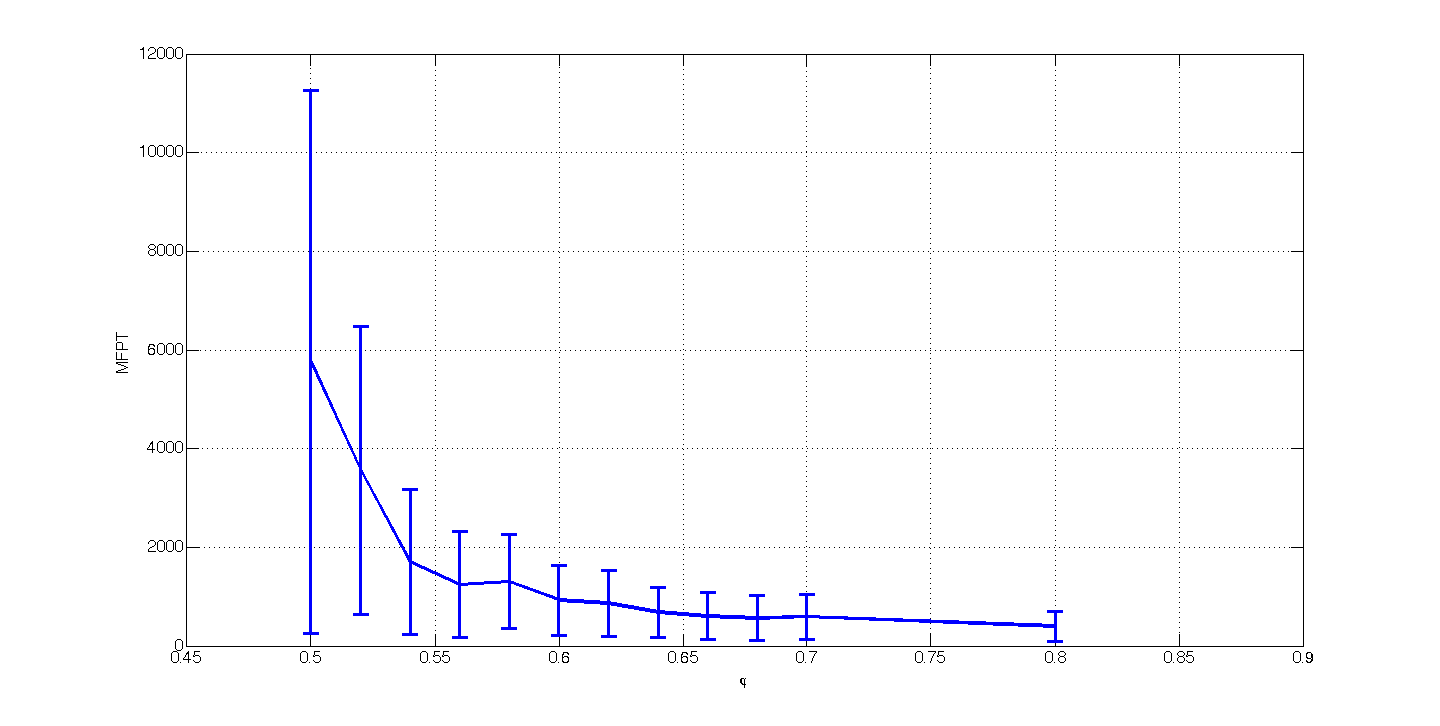
\includegraphics[width=0.85\columnwidth]{/home/harrison/Documents/mRNA/Figures_for_writeup/MFPT_phi_varied_15June_v3.png}
                \caption{MFPT as a function of $\phi$}
                \label{fig:phi}
        \end{subfigure}%
        
        
        ~ %add desired spacing between images, e. g. ~, \quad, \qquad, \hfill etc.
          %(or a blank line to force the subfigure onto a new line)
        \begin{subfigure}[h]{0.95\columnwidth}
                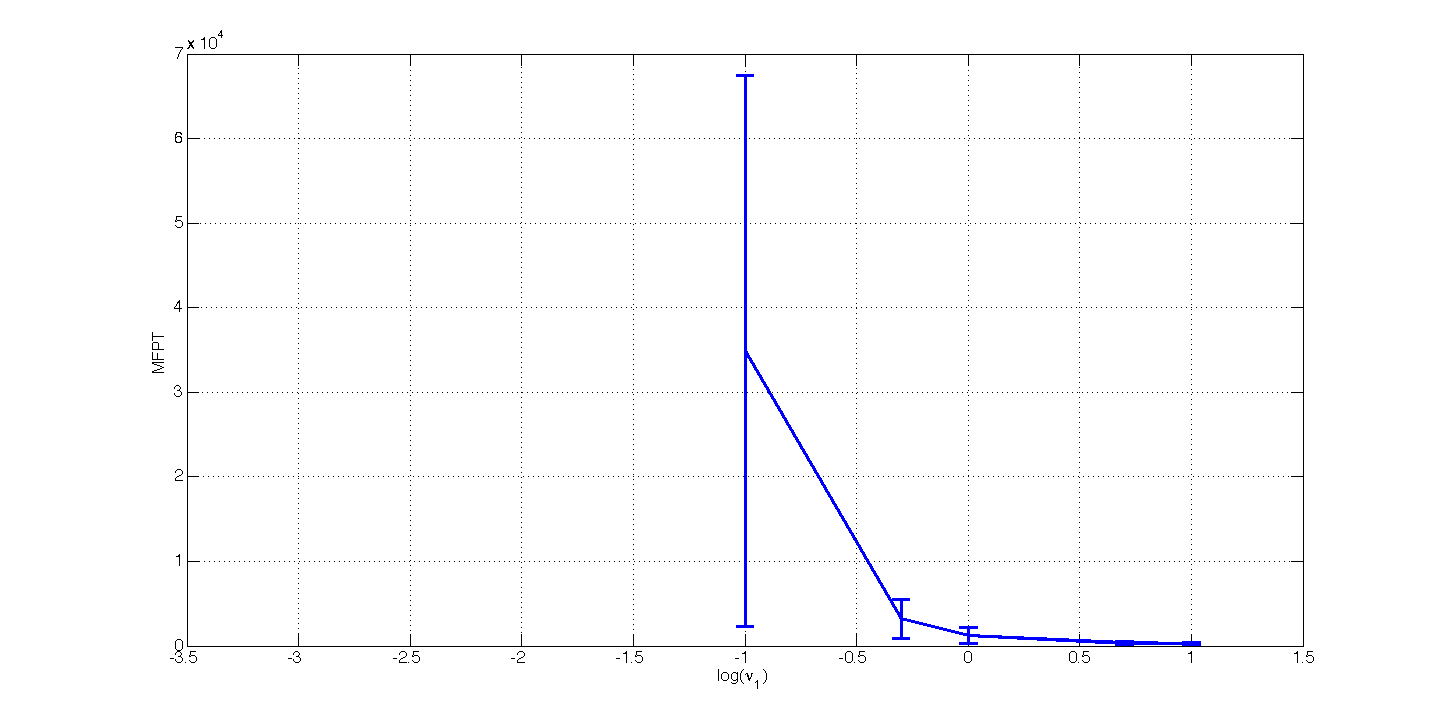
\includegraphics[width=0.85\columnwidth]{/home/harrison/Documents/mRNA/Figures_for_writeup/MFPT_nu1_varied_15June_v3.png}
                \caption{MFPT as a function of $\nu_1$ and $\nu_2$}
                \label{fig:nu1}
        \end{subfigure}
         
         ~
         
         \begin{subfigure}[h]{0.95\columnwidth}
                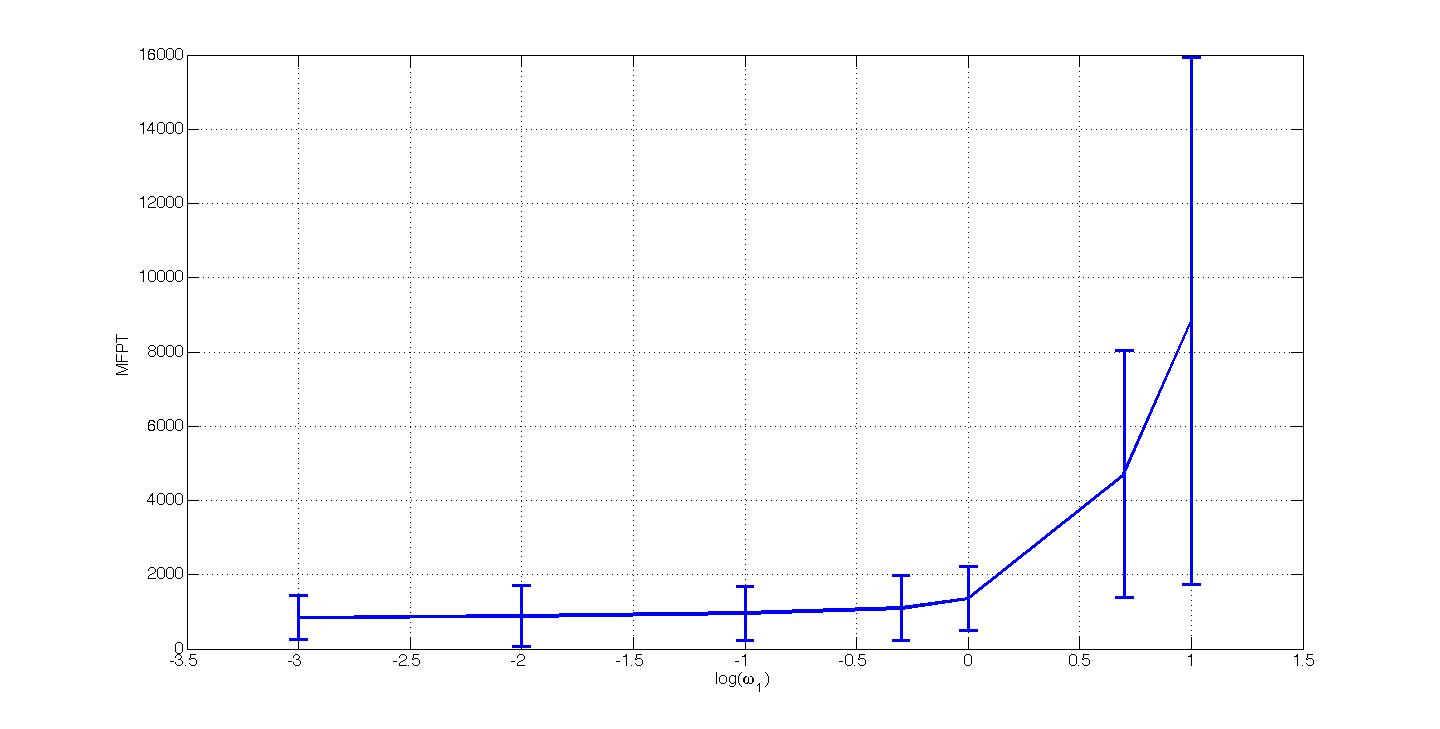
\includegraphics[width=0.85\columnwidth]{/home/harrison/Documents/mRNA/Figures_for_writeup/MFPT_omega1_varied.png}
                \caption{MFPT as a function of $\omega_1$}
                \label{fig:omega1}
        \end{subfigure}%
        
        ~ 
   
    \begin{subfigure}[h]{0.95\columnwidth}
                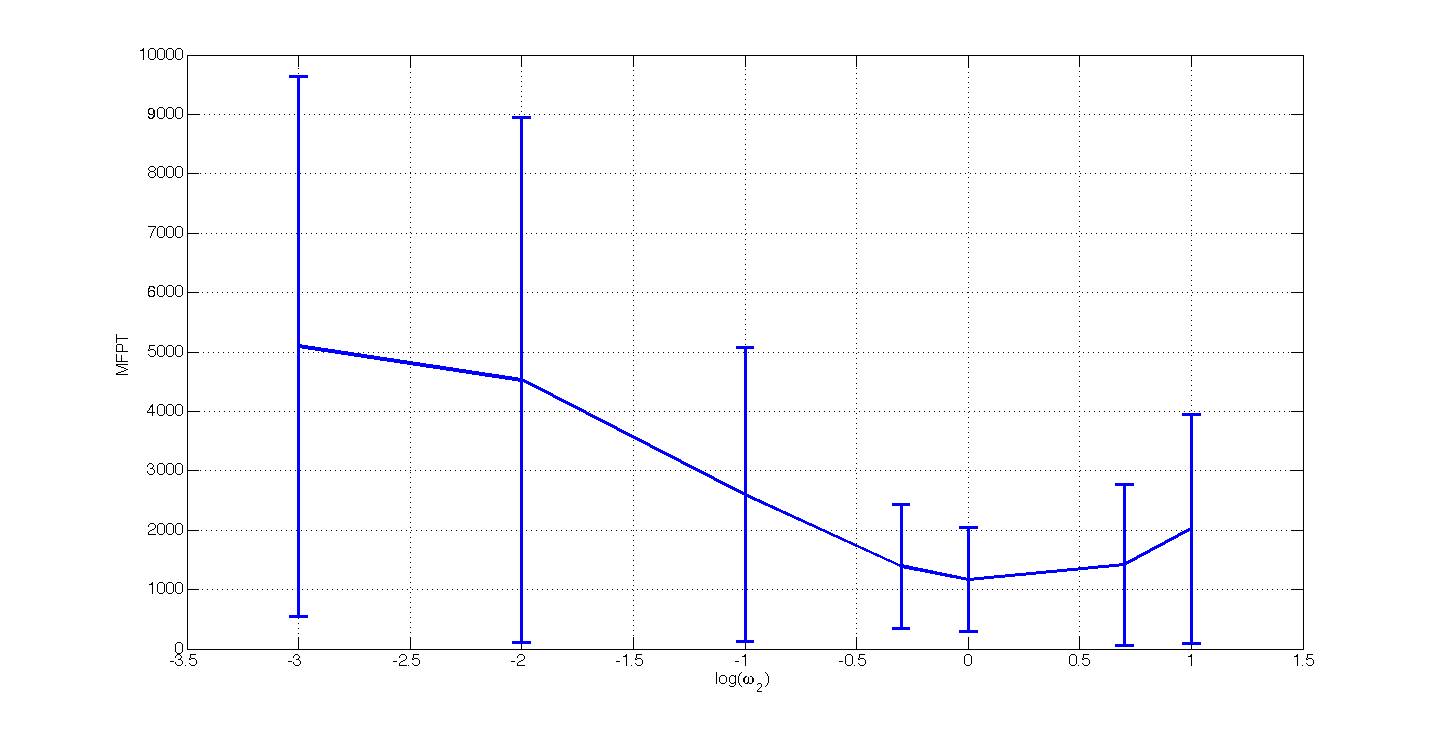
\includegraphics[width=0.85\columnwidth]{/home/harrison/Documents/mRNA/Figures_for_writeup/MFPT_omega2_varied.png}
                \caption{MFPT as a function of $\omega_2$}
                \label{fig:omega2}
        \end{subfigure}%
        
        
        ~ 
        
         \begin{subfigure}[h]{0.95\columnwidth}
                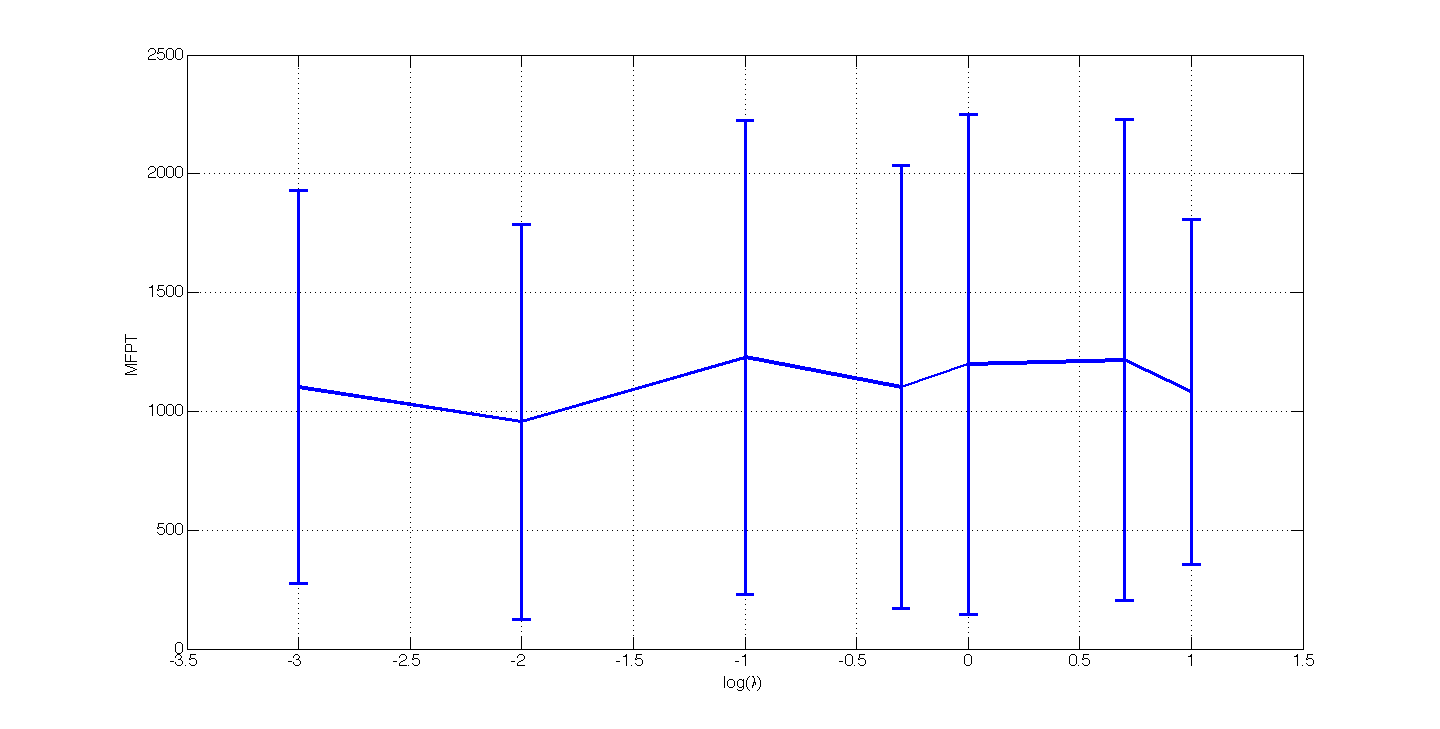
\includegraphics[width=0.85\columnwidth]{/home/harrison/Documents/mRNA/Figures_for_writeup/MFPT_lambda_varied.png}
                \caption{MFPT as a function of $\lambda$}
                \label{fig:lambda}
        \end{subfigure}%
        
        
        ~ 
        \caption{Mean first passage time (MFPT) simulated from the two phase model for parameters $\omega_1=0.42$, $\omega_2=0.84$, $\lambda=0.11$. For \ref{fig:phi}, we take $\nu_1=1.16$ and $\nu_2=0.8$ whilst varying $\phi$. 
        For \ref{fig:nu1}, we fix $\phi=0.58$ and set $\nu_2=\frac{1}{2}\nu_1$ while varying $\nu_1$. Results are averaged over 100 particles with standard deviation shown on the error bars.}
        \label{FIG:Sensitivity_analysis}
\end{figure}

Based on direct measurements from manually tracked grk-GFP mRNA complexes in \textit{Drosophila} nurse cells, we are able to make direct preliminary estimates of the parameters of our model.
All data were obtained from \citet{DavidsonPhD2015}.
Particles are classed as static, paused or active.
The number of total particles counted was $N=340$ in a 40x40 $\mu \text{m}$ area.
The proportions of particles in each of the classes is $25\%$ active, $50\%$ paused and $21\%$ static. 
Over the timescale observed, particles did not transition between states and these are proportions of particles. 
Particle speeds were assessed by observing a 10x10 $\mu \text{m}$ area for 50 timepoints, with images taken in 1 $z$ slice at 3 frames per second. 
Average speed in active transport $\nu_1 $ was  $1.163 \pm 0.08 \mu \text{ms}^{-1}$ from $n=33$. 
Average run length was $2.785 \pm 0.66 \mu \text{m}$. 
In the paused phase, an average speed, $\nu_2$, of $0.798 \pm 0.6 \mu \text{ms}^{-1}$ was observed from 58 particles with an average run length of  $0.84 \pm 0.06 \mu \text{m}$. 

Considering the process as a continuous time Markov chain, with active transport and diffusive states, we obtain that the steady state of the continuous time markov chain is $[\frac{\omega_2 }{\omega_1 + \omega_2},\frac{ \omega_1}{\omega_1+\omega_2}]$. 
Then assuming ergodicity and neglecting anchored particles, this approach gives us $\frac{\omega_2 }{\omega_1 + \omega_2} = \frac{2}{3}$ and $\frac{\omega_1 }{\omega_1 + \omega_2} = \frac{1}{3}$ by comparing to the proportions of particles observed in each state.
Therefore the rates of falling off and reattaching must be different.

Now assuming there are no internal transitions back to the active transport state, then we have $\omega_1 = 0.42 s^{-1}$ and hence $\omega_2 = 0.84 s^{-1}$. 
We can also deduce that the rate $\lambda = 0.95-0.84 = 0.11 s^{-1}$.  

This gives parameter values to use of $\nu_1 = 1.16$, $\nu_2 = 0.80$, $\omega_1 = 0.42 $, $\omega_2 = 0.84$, $\lambda = 0.11$.

Based on simulations from the model, we obtain a mean first passage time, averaged across 100 particles, of $1140s = 19\text{min}$.
Given that stage 5 in \textit{Drosophila} oocytes lasts 5 hours, this timescale for the passage time appears to be an order of magnitude shorter, suggesting that the limiting step in the transport and localization of the mRNAs is their production from the nucleus rather than the transport step.
We are also able to make predictions on what would happen if we halved the speed of the molecular motors via a genetic mutation. The resulting distribution over time would look like... and the MFPT would be...

\subsubsection{Analytics}
Is it worth doing any analytics? Is there anything worth including?

\subsection{Approximate Bayesian Computation (ABC)}
In a statistical inference context, the likelihood of data given a certain set of parameters is a central quantity. 
In particular, it is essential in calculation of the posterior over the parameters given certain data. 
The posterior is desirable as it offers more information than just point estimates of the parameters.
Although for simple models it may be possible to evaluate the likelihood analytically, often for more complex models the likelihood is not tractable or is very expensive to compute.  
Approximate Bayesian Computation (ABC) techniques have been developed to address this issue \cite{beaumont2002approximate}.
Instead of directly evaluating the likelihood, ABC techniques assume it is possible to cheaply simulate from the model and use this to approximate the likelihood.

In an ABC rejection sampling approach we follow the procedure shown in algorithm \ref{ABC-RS}, where $\pi(\theta)$ is a prior on the parameters, $\rho$ is a distance metric, $S(x)$ is a summary statistic used to summarize the data $x$ and $\epsilon$ is a maximum tolerance for acceptance. 
%The accepted parameters $\theta$ then represent an approximation to the posterior distribution. 
\begin{algorithm}
\caption{ABC Rejection Sampling}\label{ABC-RS}
\begin{algorithmic}[1]
\State \textbf{for} $i=1$ \text{to} $n$  \{
\State Sample parameters $\theta$ from a prior on those parameters $\pi (\theta)$ 
\State Simulate data $x$ from the model $M(\theta)$ using those parameters 
\State Calculate distance from observed data $y$.
\If {$\rho (S(x),S(y)) < \epsilon $} accept the parameters $\theta$
\Else \hspace{2pt} reject the parameters $\theta$.
\EndIf
\State \}
\end{algorithmic}
\end{algorithm}

One drawback of this algorithm is that it depends on appropriate choice of the distance metric $\rho$, the summary statistic $S(x)$ and the tolerance $\epsilon $. 
Clearly the quality of the posterior will depend on the choice of these hyperparameters, as for example increasing $\epsilon $ will decrease the quality of the corresponding posterior.
In some settings it may be possible to take the full data, rather than a summary statistic and to set $\epsilon=0$ which would give an exact sample from the posterior, but in general this is not possible computationally. 
We can eliminate the importance of the tolerance to some extent by simulating $N$ samples from the prior, storing all the distances and keeping the closest $\alpha$ quantile of the sampled parameters to the observed data. 
The quality of the posterior still depends on $N$ and $\alpha$ but the choice of $\epsilon $, which may be dependent on other model parameters, is removed. 

The efficiency of the rejection sampling method is low, particularly for small values of $\epsilon$ which lead to tiny acceptance rates meaning many wasted samples. 
More efficient ways of sampling possible parameters $\theta$ have been suggested including Sequential Monte Carlo and Population Monte Carlo techniques $\citep{toni2009approximate, sisson2007sequential, lenormand2013adaptive}$.
We have opted to use an adaptive Population Monte Carlo (APMC) method presented in \citet{lenormand2013adaptive}. 
This is implemented as shown in algorithm \ref{ABC-APMC}, where ...
\begin{algorithm}
\caption{ABC Adaptive Population Monte Carlo}\label{ABC-APMC}
\begin{algorithmic}[1]
\State \textbf{for} $i=1$ \text{to} $n$  \{
\State Sample parameters $\theta$ from a prior on those parameters $\pi (\theta)$ 
\State Simulate data $x$ from the model $M(\theta)$ using those parameters 
\State Calculate distance from observed data $y$.
\If {$\rho (S(x),S(y)) < \epsilon $} accept the parameters $\theta$
\Else \hspace{2pt} reject the parameters $\theta$.
\EndIf
\State \}
\end{algorithmic}
\end{algorithm}

Inference on model parameters using ABC has been successfully applied to a variety of types of model in a biological context, often helping to offer biological insight into the model system.
Cell migration models have used ABC to process data from scratch assays \citep{johnston2014interpreting} and \textit{in vivo} data \citep{liepe2012calibrating}, while individual-based ecological models with up to 14 parameters have also applied ABC for parameterisation \citep{van2015calibration}. 

When using ABC methods, it is important to be aware also of their limitations. 
It has been highlighted via \citet{robert2011lack} that although the error from the tolerance $\epsilon$ can be eliminated in the limit $\epsilon \rightarrow 0$, the use of summary statistics of the data may have larger effects, particularly when comparing models using ABC.
Some more systematic methods for choice of summary statistics have been suggested, which use minimization of certain measures of entropy to determine which summary statistics are most informative \citep{nunes2010optimal}.

\subsubsection{Dependence of weights on distance}
At each generation of the APMC algorithm, we calculate a distance for each set of parameters.
These ought to be informative for which particles should contribute most heavily to the next generation, but are not used directly in the ABC-APMC algorithm.
We have considered how we could use weights in the ABC-APMC algorithm that depend directly on the distances, using the update step: 
\begin{equation}
 w_{i}^{(t-1)} = \frac{\pi(\theta_i^{(t-1)}}{\rho_i^{(t-1)}} \frac{ w_i^{(t-1)} }{\sum_{j=1}^{N_{\alpha}} w_j^{(t-1)} }. 
\end{equation}                                                                                                                                                       
However, the weights used in the ABC-APMC algorithm are required to ensure that the importance sampling is performed correctly when sampling from the weighted distribution at the next time step.
Without this exact choice, there is no gauruntee that the resulting posterior would be unbiased.
Although heuristically, these weights seem an attractive option, statistically they may result in poor quality posteriors.

\section{Results and Discussion}
\subsection{Evaluation of ABC methods on in silico data}
We demonstrate the effectiveness of the ABC inference techniques on in silico data, before applying them directly to real data sets. 
We present first the results of applying ABC methods to our model with a broad prior and known parameter values, as shown in figure \ref{FIG:ABC_Posterior}.
\begin{figure} 
        \centering
        \begin{subfigure}[h]{0.95\columnwidth}
                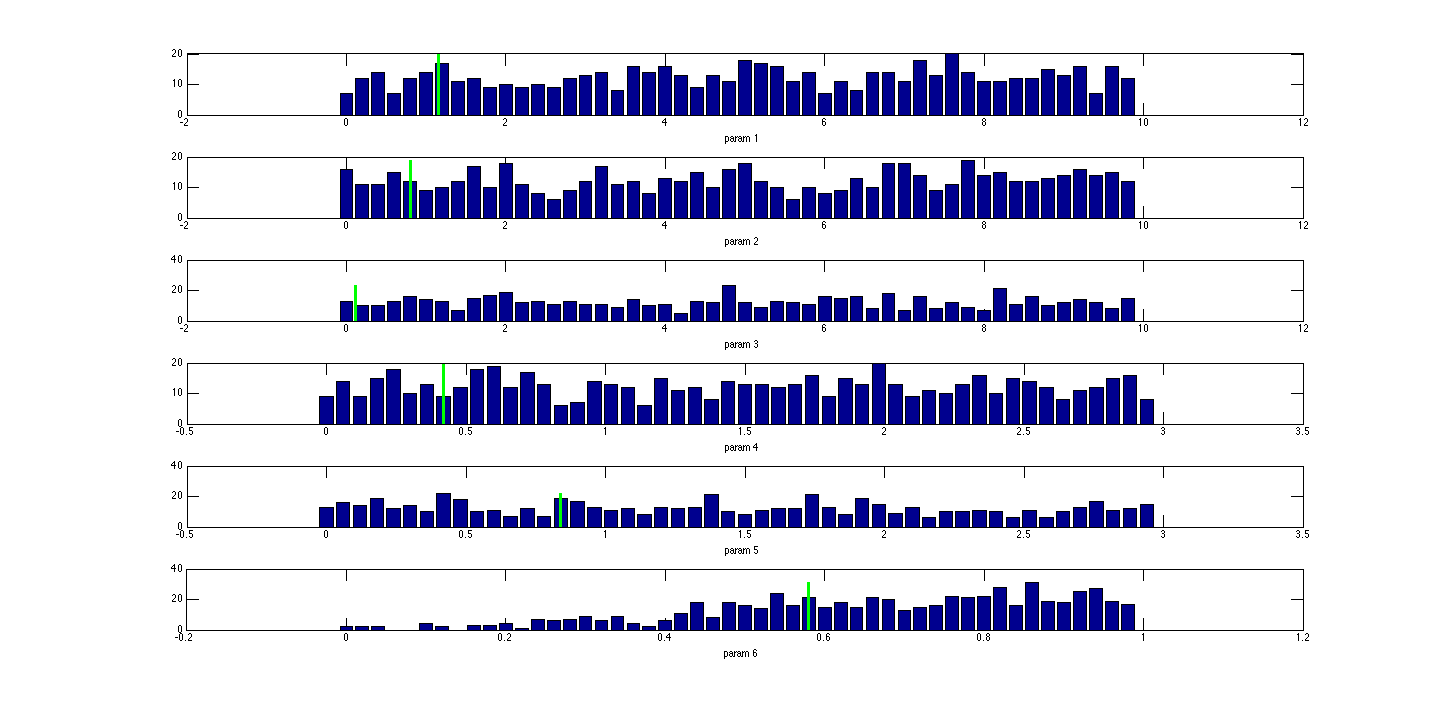
\includegraphics[width=\columnwidth]{/home/harrison/Documents/mRNA/Figures_for_writeup/Posterior_all_params_N100_paccmin001.png}
                \caption{Posterior obtained for $N=100$}
                \label{fig:a}
        \end{subfigure}%
        
        
        ~ %add desired spacing between images, e. g. ~, \quad, \qquad, \hfill etc.
          %(or a blank line to force the subfigure onto a new line)
        \begin{subfigure}[h]{0.95\columnwidth}
                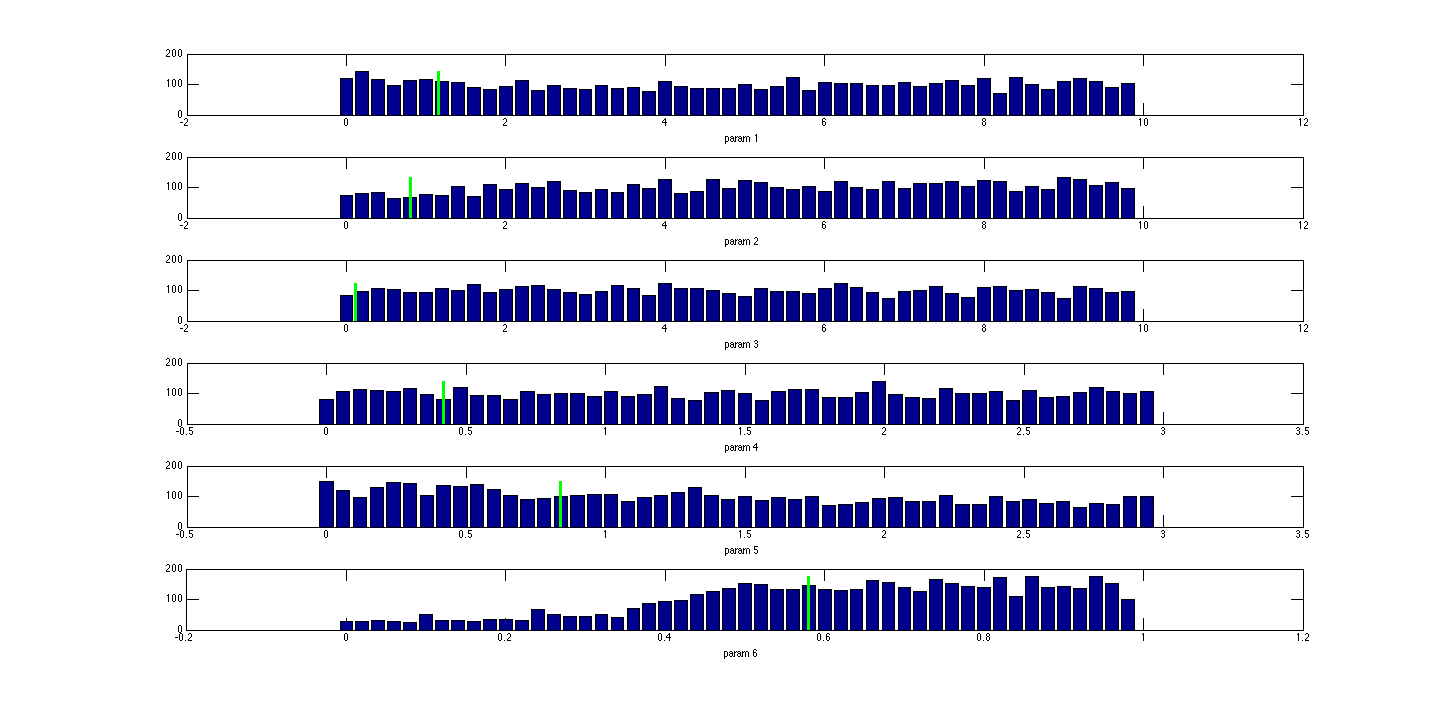
\includegraphics[width=\columnwidth]{/home/harrison/Documents/mRNA/Figures_for_writeup/Posterior_all_params_noninformative.png}
                \caption{Posterior obtained for $N=5000$}
                \label{fig:b}
        \end{subfigure}
        \caption{Posterior for each parameter approximated via ABC methods, using $N=100$, $\alpha=0.5$, $n_{repeats}=5$. For \ref{fig:a}, the minimum acceptance probability was set at $p_{accmin} = 0.01$, whereas for \ref{fig:b} $p_{accmin} = 0.1$ was used.}
        \label{FIG:ABC_Posterior}
\end{figure}

For each experiment, we simulate a data set from chosen parameters and evaluate its summary statistic. 
That summary statistic is compared to summaries of data generated from proposed parameters, as described above.
We average the results obtained across a number of experiments denoted $n_{repeats}$.
As summary statistics we take the spatial distribution of the cargoes averaged in the $x$ direction at given times $t_1,t_2,t_3$ and use a symmetric version of the Kullback-Leibler divergence as our distance to compare distributions.
Uniform priors are used for each parameter between biologically realistic maximum and minimum values.
In figure \ref{In_silico_1}, the contours of the pairwise parameter distributions are shown. 
In table (1), we present the results of varying the parameters $N, n_{repeats}, \alpha, p_{acc_{min}}$ on the quality of the posteriors.

Explain the set up.
Which method performs best? Is this consistent?
Why might this be?

\subsection{Application of ABC to \textit{Drosophila} nurse cell data}
We collected some data.
What did we collect? Why? Might it have been more informative if we could have collected something else?
Why didn't we do that?
What estimates for the posterior of the parameters do we get from ABC?
Are these informative?
Do they agree with what we obtained by direct measurement? Why?

\section{Conclusion}
Through use of a model based approach of mRNA transport and localization, we have been able to represent the dynamics of this process and reproduce behaviour observed experimentally.
We constructed a velocity jump process with two phases of motion to represent motion in active transport and in diffusion.
Since simulation from this model was accessible but the likelihood was intractable, we employed ABC methods to infer the parameters from our model from data collected via live \textit{in vitro} imaging and compared the results of this with values obtained from direct measurement.

The timescales for mean first passage times based on simulations from the model are on the order of tens of minutes, rather than hours for the inferred parameters, suggesting that the transport step is not the rate limiting stage of the mRNA localization process.
Based on the modelling work presented here, we postulate that the production of mRNA in the nucleus of the nurse cells is instead the rate limiting stage.

\subsection{Further work}
The subcellular environment is in some ways drastically different to that assumed in our spatially homogeneous two dimensional model.
In reality, cells exist in three dimensions and are crowded inside with a hetrogeneous environment. 
One possible method of representing heterogeneity in the cell would be by use of a potential to account for volume exclusion effects, as used by \citet{isaacson2011influence} in the context of nuclear export of mRNAs.
The three dimensional nature of the environment presents further challenges for tracking, as RNPs move between frames.
Although some progress has already been made in this area \citep{thompson2010three}, we hope that incorporation of modelling into a tracking framework could enable tracking of particles over longer timescales at increased resolution. 
Motivated by a Kalman filter type approach \citep{faragher2012understanding}, we would like to investigate further using our model combined with regular inputs of data over time to assist particle tracking algorithms in the linkage step of tracking.
Therefore in future the model should be extended to enable us to capture behaviour in three dimensions. 


\section*{SUPPLEMENTARY MATERIAL}

An online supplement to this article can be found by visiting BJ Online at http://www.biophysj.org.

\vspace{1cm}
\footnotesize The authors would like to acknowedge valuable discussions from Dr S. Filippi and Dr J. Rittscher, in addition to beneficial input from Prof I. Davis.


% Here references are directly included this tex file.
% But we can generate reference list from bibliography database
% Compile and format the bibliography (bj_bibtex_template.bib BibTeX
% file must be present in the document directory)

%The source file for this document is called
%\emph{biophys\_latex\_template.tex}.  Apart from this \LaTeX\ file, you
%will also need the bibliography file, the \BibTeX\ style file, and the
%EPS and PDF figure files.

%See the bibliography file \emph{bj\_bibtex\_template.bib} for the
%literature data.  It was mostly generated from the saved
%text-formatted PubMed entries using the \emph{med2bib} program and
%edited by the \emph{tkbibtex} or directly in the \emph{emacs} editor.

%The \emph{biophysj.bst} file is a \BibTeX\ style file that contains
%information about the format required by Biophysical Journal for the
%list of references.


%\bibliography{bj_bibtex_template}

% Bibliography style (requires the style file biophysj.bst in the
% document directory)
\bibliographystyle{biophysj}
\bibliography{my_citations.bib}

% Figure legends
%%Automatically it will add the figure legends  and table legends as a list by below command


\newpage

\listoffigures

\newpage

\listoftables

% Figures and Tables coding should be placed where the
% first reference in the text.
% All the Figure files should be placed same working directory,
% for example (fig_1.eps and fig_1.pdf files must be present
% in the document directory)

% closing statement, nothing below matters

\end{document}
